\documentclass{standalone}
\usepackage{pgfplots}
\pgfplotsset{compat=1.13}
\usepackage{amsmath}

\newcommand{\aalpha}{\boldsymbol{\alpha}}

\begin{document}

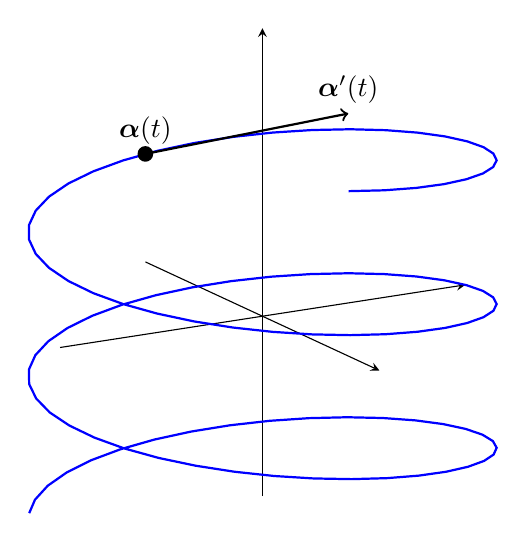
\begin{tikzpicture}%
    \begin{axis}[
            view={60}{15},
            width=0.8\textwidth,
            height=0.8\textwidth,
            axis lines=center,
            xlabel=$ $,ylabel=$ $,zlabel=$ $,
            zmin=-1, zmax=1.6,
            xtick=\empty,  ytick=\empty,  ztick=\empty
        ]
        \addplot3[blue,thick,domain=-9:8,samples=101,samples y=0]
        ({sin(deg(x))},
        {cos(deg(x))},
        {2*x/(5*pi)});
        \draw[->,thick] (axis cs:-1,0,0.6) -- (axis cs:-1,1,0.65) node[anchor=south]{\(\aalpha'(t)\)};
        \node[circle,fill,inner sep=2pt] at (axis cs:-1,0,0.6) {} ;
        \node[anchor=south] at (axis cs:-1,0,0.6) {\(\aalpha(t)\)} ;
    \end{axis}
\end{tikzpicture}

\end{document}